\documentclass[a4paper, twoside]{report}

%%%%%%%%%%%%%%%%%%%%%%%%%%%%%%%%%%%%%%%
%%%%%%%%%%%%% IMPORT PACKAGES %%%%%%%%%
%%%%%%%%%%%%%%%%%%%%%%%%%%%%%%%%%%%%%%%
\usepackage[hidelinks]{hyperref}
\usepackage{subfigure}
\usepackage{fancyvrb}
\usepackage{amsmath, amsfonts, amsthm, amssymb}
\usepackage{stmaryrd}
\usepackage{verbatim}
\usepackage{graphicx}
\usepackage{setspace}
\usepackage[ruled, vlined]{algorithm2e}
\graphicspath{{Figures/}}

%%%%%%%%%%%%%%%%%%%%%%%%%%%%%%%%%%%%%%%5
\usepackage{listings}
\usepackage{xcolor}
\definecolor{codegreen}{rgb}{0,0.6,0}
\definecolor{codegray}{rgb}{0.5,0.5,0.5}
\definecolor{codepurple}{rgb}{0.58,0,0.82}
\definecolor{backcolour}{rgb}{0.95,0.95,0.92}

\lstdefinestyle{mystyle}{
    backgroundcolor=\color{backcolour},   
    commentstyle=\color{codegreen},
    keywordstyle=\color{magenta},
    numberstyle=\tiny\color{codegray},
    stringstyle=\color{codepurple},
    basicstyle=\ttfamily\footnotesize,
    breakatwhitespace=false,         
    breaklines=true,                 
    captionpos=b,                    
    keepspaces=true,                 
    numbers=left,                    
    numbersep=5pt,                  
    showspaces=false,                
    showstringspaces=false,
    showtabs=false,                  
    tabsize=2
}
\lstset{style=mystyle}
%%%%%%%%%%%%%%%%%%%%%%%%%%%%%%%%%%%%%%%%
%%%%%%%%%%%%%%%%%%%%%%%%%
\newtheorem{theorem}{Theorem}[section]
\newtheorem{exa}{Example}[section]
\newtheorem{corollary}[theorem]{Corollary}
\newtheorem{lemma}[theorem]{Lemma}
\newtheorem{proposition}[theorem]{Proposition}

\theoremstyle{definition}
\newtheorem{definition}[theorem]{Definition}
\newtheorem{remark}[theorem]{Remark}
\newtheorem{notation}[theorem]{Notation}
\newtheorem{assumption}[theorem]{Assumption}
\newtheorem{conjecture}[theorem]{Conjecture}

\newcommand{\ind}{1\hspace{-2.1mm}{1}} %Indicator Function
\newcommand{\I}{\mathtt{i}}
\newcommand{\D}{\mathrm{d}}
\newcommand{\E}{\mathrm{e}}
\newcommand{\RR}{\mathbb{R}}
\newcommand{\sgn}{\mathrm{sgn}}
\newcommand{\atanh}{\mathrm{arctanh}}
\def\equalDistrib{\,{\buildrel \Delta \over =}\,}
\numberwithin{equation}{section}


%%%%%%%%%%%%%%%%%%%%%%%%%%%%%%%%%%%%%%%%%%%%%%%
%%%%%%%%%%%%%%%%%%%%%%%%%%%%%%%%%%%%%%%%%%%%%%%
%% Sets page size and margins
\usepackage[a4paper,top=3cm,bottom=2cm,left=3cm,right=3cm,marginparwidth=1.75cm]{geometry}
\title{Solving the Collatz conjecture}
\author{Ilia Sobakinskikh  (CID: 00000000)}

\begin{document}
\begin{titlepage}

\newcommand{\HRule}{\rule{\linewidth}{0.5mm}} 

\includegraphics[width=8cm]{logo.png}\\[1cm]
\center

\quad\\[1.5cm]
\textsc{\Large Imperial College London}\\[0.5cm]
\textsc{\large Department of Mathematics}\\[0.5cm]

\makeatletter
\HRule \\[0.2cm]
\begin{spacing}{2.5}
{\huge \bfseries \@title}
\end{spacing}
\HRule \\[1.5cm]
 
\begin{minipage}{0.8\textwidth}
\begin{flushleft} \large
\emph{Author:}
\@author
\end{flushleft}
\end{minipage}
~\vspace{2cm}
\makeatother


{\large A thesis submitted for the degree of}\\[0.5cm]
{\large \emph{MSc in Mathematics and Finance, 2022-2023}}\\[0.5cm]

\vfill

\end{titlepage}

\mbox{}\newline\vspace{10mm} \mbox{}\LARGE
%
{\bf Declaration} \normalsize \vspace{5mm}

The work contained in this thesis is my own work unless otherwise stated.

\newpage

\renewcommand{\abstractname}{Acknowledgements}
\begin{abstract}
    This is where you usually thank people who have provided useful assistance, feedback,...., during your project.
\end{abstract}

\newpage

\renewcommand{\abstractname}{Abstract}
\begin{abstract}
    The abstract is a short summary of the thesis' contents.
    It should be about half a page long and be accessible by someone not familiar with the project.
    The goal of the abstract is also to tease the reader and make him want to read the whole thesis.
\end{abstract}

\tableofcontents
\listoffigures
\listoftables






% %%%%%%%%%%%%%%%%%%%%%%%%%%%%%%%%%%%%%%%%%%%%%%%
% \begin{remark}
% Please bear in mind the following when writing your thesis (or anything for that matter):
% you are not writing for you. You are writing for an audience, who will (have to) read your work.
% Please be considerate, and explain everything clearly. 
% In this case, the audience could be your fellow MSc students, 
% with some general knowledge of the area, but maybe not specialised to your particular topic.
% \end{remark}


% \newpage
% %%%%%%%%%%%%%%%%%%%%%%%%%%%%%%%%%%%%%%%%%%%%%
% \chapter{How to write mathematics}\label{sec:HowTo}
% In this section, we show some examples of properly written mathematical expressions and sentences.
% In the header of your thesis, you can define \LaTeX \ shortcuts to write more quickly.


%%%%%%%%%%%%%%%%%%%%%%%%%%%%%%%%%%%%%%%%%%%%%%%
\chapter*{Introduction}

% The introduction is one of the most important components of the thesis.
% It should be readable by anyone, 
% including people without prior knowledge of the field.
% It should progressively introduce the main topic of the paper, and explain the structure of the thesis.
% In Section~\ref{sec:HowTo}, we shall provide several examples of clearly written examples,
% whereas Section~\ref{sec:WhatNotToDo} will gather a certain number of common mistakes and errors.

In this thesis, we explore how the inference time of a Transformer Neural Network can be efficiently optimized with applications to real-time anomaly detection in financial time series.
The financial time series are price series such as asset prices.
Unfortunately, the data is often with errors or outliers that make the downstream data processing tasks useless, unstable or even harmful \cite{Falkenberry_2008} \cite{Vallis_Hochenbaum_Twitter}. Moreover, the amount of financial time-series data has been significantly increasing \cite{AnomalyDataBig}.
Hence, there is a need for better data-cleaning methods in terms of accuracy and in terms of processing speed.

Transformers as a neural network architecture have achieved superior performances in many tasks such as Natural Language Processing and Computer Vision \cite{TransformersNLP}.
Time series modelling and especially anomaly detection tasks can benefit from the features of transformers architecture in multiple ways, including the capacity to capture long-range dependencies and interactions \cite{2202.07125}.

Increasingly powerful hardware, such as field-programmable gate arrays (FPGAs), have seen increasing usage in recent years due to their reconfigurability and high performance \cite{10.1007/978-3-319-56258-2_14}.

We explore different Transformer architectures for time series modelling and how they can be efficiently implemented on an FPGA board (PYNQ-Z2).
In particular, we examine the application of Transformers to detect anomalies in time series and we show how they can be efficiently implemented on an FPGA board to minimize latency or to maximize throughput.


%%%%%%%%%%%%%%%%%%%%%%%%%%%%%%%%%%%%%%%%%%%%%%%
\chapter{Methodology}

In this chapter, we will describe the main concepts and ideas used in this work.
The reader will be introduced to the main concepts of the Transformer architecture and how it can be used for anomaly detection in time series.
Finally, the main concepts of programming an FPGA will be introduced and the specific optimizations that can be applied to speed up the computations.

% TODO: use neurips paper as an example:
% https://proceedings.neurips.cc/paper_files/paper/2019/file/6775a0635c302542da2c32aa19d86be0-Paper.pdf

\section{Problem Formulation}


\begin{definition}
    We consider a \textbf{time-series} $\mathcal{T}$ which is simply a timestamped sequence of observations $x_i \in R^n$.
\end{definition}
\begin{remark}
    Most of the times we will consider univariate case, i.e. $n=1$.
    An example of this is a price time-series of a single stock.
    However, the multivariate case is also important and we will consider it in the experiments.
    For example, one can consider a time-series of prices of multiple stocks to get a multivariate time series.
\end{remark}


\begin{definition}
    The \textbf{Anomaly Detection} task:
    for any time-series $\hat{\mathcal{T}}$ of length $n$, we need to predict $\mathcal{Y} = \{y_1, . . . , y_n \}, y_i \in \{0, 1\}$,
    whether the datapoint at the $i$-th timestamp anomalous (where by convention we will use $1$ as anomaly and $0$ as not an anomaly).
\end{definition}
In this work, we will restrict ourselves to the \textbf{supervised case}
where the labels $y_i$ are known for the \emph{seen} (or training) part of the dataset.

\begin{remark}
    One can also consider an unsupervised task.
    However, one issue with the unsupervised task is that it is hard to evaluate
    the performance (i.e., accuracy) of the model's predictions \cite{1905.05667}.
\end{remark}


\section{Transformers}

In this section, we will describe the main concepts of the Transformer architecture.
We will describe the main building blocks of the Transformer architecture
and will give a special treatment to the attention mechanism firstly introduced in \cite{1409.0473}.

% TODO:
% https://ai.stackexchange.com/questions/23221/how-is-bert-different-from-the-original-transformer-architecture
% Both the encoder-decoder architecture and the attention mechanism are not novel proposals. In fact, previous neural network architectures to solve many NLP tasks, such as machine translation, had already used these mechanisms (for example, take a look at this paper). The novelty of the transformer and this cited paper is that it shows that we can simply use attention to solve tasks that involve sequences (such as machine translation) and we do not need recurrent connections, which is an advantage, given that recurrent connections can hinder the parallelization of the training process.

\subsubsection{General architecture}

In \cite{1706.03762}, authors introduced the Transformer architecture which a neural network architecture
which is the architecture that is dominantly used in Natural Language Processing tasks.
The architecture's main feature was reliance on the attention mechanism and the complete elimination
of recurrent and convolutional layers.

\begin{figure}[h!]
    \centering
    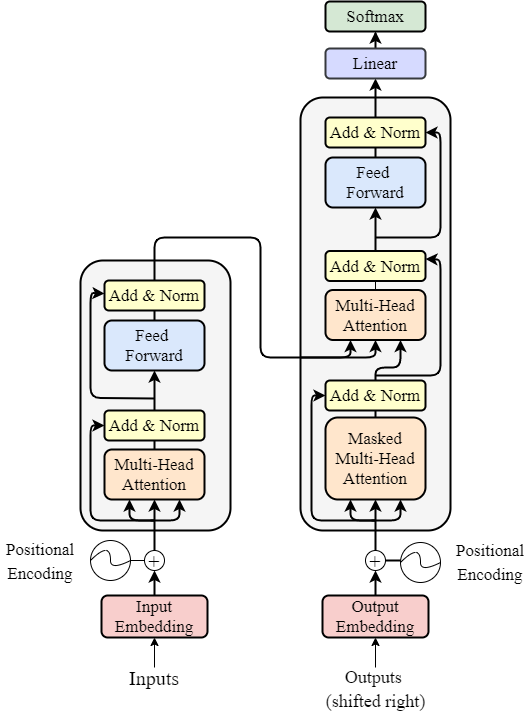
\includegraphics[scale=0.5]{attention_is_all_you_need.png}
    \caption{Model architecture of the Transformer \cite{1706.03762}}
    \label{fig:attention_is_all_you_need}
\end{figure}

Figure \ref{fig:attention_is_all_you_need} presents the main architecture of the transformer.
The architecture consists of an \textbf{encoder} and a \textbf{decoder}.
For the purpose of the thesis we will only consider the \textbf{encoder} part of the architecture.
% TODO: maybe describe the decoder also?
The \textbf{encoder} is preceded by a \textbf{positional encoding} layer which is used to \emph{inject} the positional information
to the input vectors $x_i$ because the attention mechanism is permutation invariant, this will be explained in Section \ref{sec:attention_mechanism}.

% TODO: explain positional encoding and why we need it
% https://uvadlc-notebooks.readthedocs.io/en/latest/tutorial_notebooks/tutorial6/Transformers_and_MHAttention.html

The \textbf{encoder} consists of $N$ identical layers. Each layer has two sub-layers which are a
\textbf{multi-head self-attention} layer and
a \textbf{feed-forward} layer.
The \textbf{feed-forward} layer $\text{FFN}(\cdot)$ is a simple fully-connected layer
with a non-linear activation function applied element-wise to the
result\footnote{
    In general, a \textbf{fully-connected} layer $\text{FC}(x)$ is simply a linear transformation inputs $X$ (i.e., a matrix multiplication) with the activation function applied element-wise to the result.
    That is, $\text{FC}(x)=f(W\cdot x + b)$ where $W$ is a weight matrix and $b$ is a bias vector and $f(\cdot)$ is the activation function.
    Authors of \cite{1706.03762} used the ReLU activation function
}.
Specifically, authors of \cite{1706.03762} used an $\text{FC}$ layer with
the ReLU activation function $$\text{ReLU}(x)=\max(0, x)$$
followed by another $\text{FC}$ layer without activation function, i.e.
$$\text{FFN}(x)=W_2 \cdot ReLU(W_1\cdot x+b_1)+b_2$$

The \textbf{Add \& Norm} layer is a residual connection \cite{1512.03385} followed by a layer normalization layers \cite{1607.06450}.
Those layers are not essential for this work and will not be described in detail.
% TODO: maybe describe them in appendix

This constitutes the main building block of the Transformer encoder architecture.
The next section will describe the attention mechanism in detail.


\subsection{Attention mechanism} \label{sec:attention_mechanism}

This section will describe the attention mechanism, its variations and the intuition behind it.
Moreover, we will compare different attention mechanism implementations in terms of
their computational complexity and their ability to capture long-range dependencies.
% basically, a survey...

\subsubsection{Dot-Product Attention and Multi-Head Attention}

% TODO: cite the common dot-product attention not as a scaled dot product attention
% https://lilianweng.github.io/posts/2018-06-24-attention/

The attention mechanism introduced in the Transformer architecture \cite{1706.03762} used a \textbf{scaled dot-product attention}.

% TODO: cite similarity to non-local filters
% Self-attention is a type of attention mechanism where the model
% makes prediction for one part of a data sample using other parts
% of the observation about the same sample. Conceptually, it feels quite similar
% to non-local means. Also note that self-attention is permutation-invariant;
% in other words, it is an operation on sets.

The main idea of the \textbf{dot-product attention} mechanism is to compute the mapping of a query $q_i$ for each input vector $x_i$ to a set of key-value pairs $(k_j, v_j)$.
The query $q_i$, key $k_i$ and value $v_i$ vectors are simply linear transformations of the input vectors $x_i$,
i.e., $q_i=W_Q\cdot x_i$, $k_i=W_K\cdot x_i$, $v_i=W_V\cdot x_i$ where $W_Q$, $W_K$ and $W_V$ are the weight matrices.
The attention mechanism is a weighted sum of the values $v_j$ where the weights are computed as a function of the query $q_i$ and the key $k_j$.
That is, $Attention(x_i)=\sum_j \alpha_{ij} v_j$ where $\alpha_{ij}=\text{softmax}(q_i \cdot v_i)$ is the weight of the $j$-th value $v_j$.
In practice, the attention mechanism is computed for all the queries $q_i$ at the same time by utilizing the following expression in matrix form:
\begin{equation}
    \begin{array}{rll}
        Q & = W_Q \cdot X, \\
        K & = W_K \cdot X, \\
        V & = W_V \cdot X
    \end{array}
\end{equation}
\begin{equation}\label{eq:dot_product_attention_matrix}
    \text{Attention}(Q, K, V)=\text{softmax}(Q K^T) V
\end{equation}

\begin{remark}
    In \cite{1706.03762}, authors additionally scaled the weights $\alpha_i$ by the square root of the dimension of the key vectors $d_k$.
    This is, however, not strictly necessary and is done for numerical stability reasons.
\end{remark}

The \textbf{multi-head attention} mechanism is simply a concatenation of multiple attention mechanisms.
That is, we can compute $h$ different attention mechanisms in parallel and then concatenate the results.
The main idea behind this is that different attention mechanisms can learn different features of the input vectors.

Figure \ref{fig:attention_is_all_you_need} visualizes the attention mechanism introduced in \cite{1706.03762}.

\begin{figure}[h!]
    \centering
    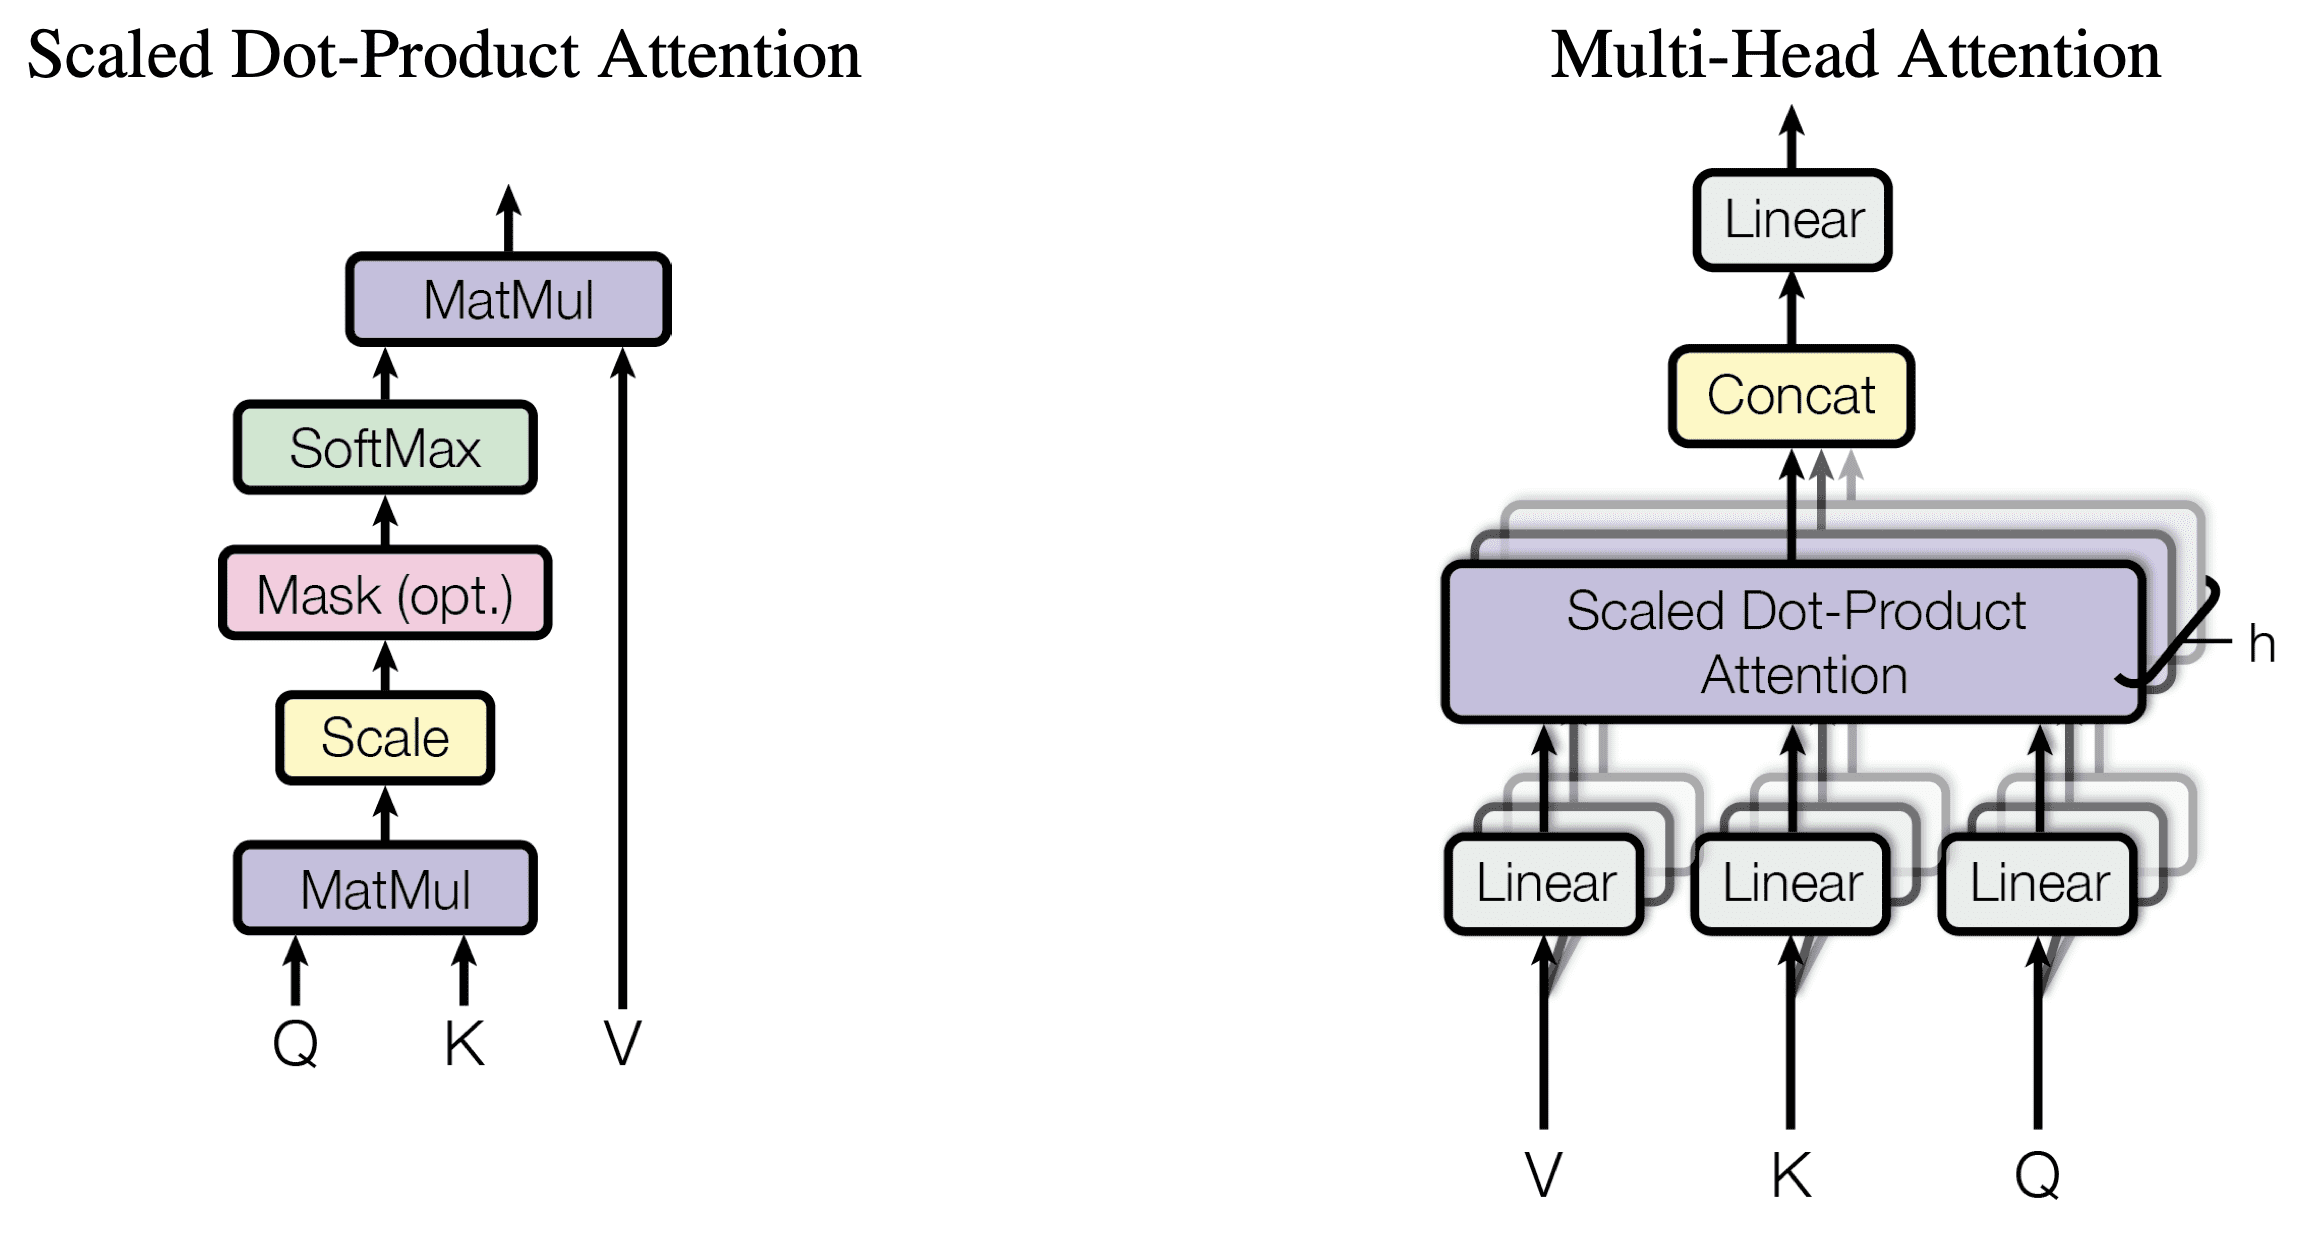
\includegraphics[scale=0.15]{scaled_dot_product_attention.png}
    \caption{Scaled Dot-Product Attention and Multi-Head Attention \cite{1706.03762}}
    \label{fig:scaled_dot_product_attention}
\end{figure}




\subsubsection{Linear attention}

In \cite{2006.16236}, authors propose an extension to the dot-product attention mechanism called \textbf{linear attention}.
This significantly reduces the computational complexity of the attention mechanism by eliminating the need to compute the softmax function.

Notice that in \ref{eq:dot_product_attention_matrix}, the softmax function is applied rowwise to the matrix $Q K^T$.
The softmax function can be substituted with a general similarity function $\text{sim}(\cdot, \cdot)$ between a query $q_i$ and a key $k_j$.
The equation \ref{eq:dot_product_attention_matrix} for output value $v'_i$ can then be rewritten as follows:
\begin{equation}
    v'_i=\text{Attention}(Q, K, V)_i=\frac{\sum_j \text{sim}(q_i, k_j) v_j}{\sum_j \text{sim}(q_i, k_j)}
\end{equation}

% TODO: maybe explain the kernel trick...
% https://en.wikipedia.org/wiki/Kernel_method
The only constrained imposed on the similarity function $\text{sim}(\cdot, \cdot)$ is that it should be non-negative for it to define an attention function.
This conveniently includes all kernels. That is $\text{sim}(q_i, k_j)=\phi(q_i)^T \phi(k_j)$ where $\phi(\cdot)$ is a feature map.

So that given a kernel with a feature map $\phi(\cdot)$, the attention mechanism can be computed as follows:
\begin{equation}
    v'_i=\text{Attention}(Q, K, V)_i=\frac{\sum_j \phi(q_i)^T \phi(k_j) v_j}{\sum_j \phi(q_i)^T \phi(k_j)}
\end{equation}

And we can rewrite the attention mechanism in matrix form as follows:
\begin{equation}
    \text{Attention}(Q, K, V)=\frac{\phi(Q)^T \phi(K) V}{\phi(Q)^T \phi(K)}
\end{equation}

Regrouping the terms, we get the following expression for the attention mechanism:
\begin{equation}
    \text{Attention}(Q, K, V)=\phi(Q)^T \frac{\phi(K) V}{\phi(Q)^T \phi(K)}
\end{equation}

% TODO: maybe rewrite with an example so that it is even more evident for the reader?...
which makes it evident that we can compute $\sum_j \phi(k_j) v_j$ once and reuse them for all the queries $q_i$
which reduces the computational complexity from $O(N^2)$ to $O(N)$ where $N$ is the number of input vectors
in the attention layer.

\begin{remark}
    In \cite{2006.16236}, authors used the $\phi(x)=elu(x)+1$ feature map where
    $elu(x)=\max(0, x)+\min(0, \alpha(\exp(x)-1))$ is the exponential linear unit activation function.
    This feature map is used to ensure that the attention mechanism is non-negative
    and hence defines a valid attention function. Moreover, $elu(\cdot)$ is used instead of $ReLU(\cdot)$
    to ensure the differentiability when x is negative.
\end{remark}


% TODO: compare to other competitors for attention layer
% https://uvadlc-notebooks.readthedocs.io/en/latest/tutorial_notebooks/tutorial6/Transformers_and_MHAttention.html
% convolutional, etc.


% TODO: different architectures from lilian weng blog, retformer, the TF in TS survey.
% describe different attention mechanisms
% https://uvadlc-notebooks.readthedocs.io/en/latest/tutorial_notebooks/tutorial6/Transformers_and_MHAttention.html
% http://nlp.seas.harvard.edu/annotated-transformer/
% https://peterbloem.nl/blog/transformers
% lilian weng


\subsection{Transformers for time series modelling}

TODO: provide the main overview of the papers that use transformers for time series modelling,
the comparison to other methods, the comparison of different transformer architectures specifically
tailored for time-series


%%%%%%%%%%%%%%%%%%%%%%%%%%%%%%%%%%%%%%%%%%%%%%%
\section{FPGA design}

% Main xilinx docs:
% https://docs.xilinx.com/r/en-US/ug1399-vitis-hls/Summary?tocId=xCTL3tR5AjP_FFYmRfl81Q

In this section, the main design principles of programming an FPGA board will be described. Readers will be introduced to the common optimization techniques and how they are achieved. The FPGA programming will be done using C++ HLS which is converted to verilog code.

\subsection{Introduction to FPGA}

% for efficient implementation reference:
% https://pytorch.org/tutorials/intermediate/scaled_dot_product_attention_tutorial.html?utm_source=whats_new_tutorials&utm_medium=scaled_dot_product_attention_tutorial

% TODO: maybe rewrite
The progress of hardware acceleration devices like field-programmable gate arrays (FPGAs) enables the achievement of high component density and low power consumption, all the while minimizing latency \cite{10.1007/978-3-319-56258-2_14}. They are commonly used to accelerate high-performance, computationally intensive systems (for example, data centers) or to minimize the latency of execution (for example, in high-frequency trading).

\subsection{FPGA development and HLS}

\subsubsection{Common Terms}

% good guide:
% https://wiki.york.ac.uk/display/RTS/Vitis+HLS+Knowledge+Base


\subsubsection{Simulation, Cosimulation}

% TODO
A way to design and debug the solution without running it on the board.

\subsubsection{HLS synthesis}

In this section, HLS synthesis will be described ~\cite{AMD2023VitisHLS}. It is now the common workflow in the FPGA development because it significantly improves the productivity when working with design.


\subsection{Common optimizations}

In this section, common optimization techniques and how they are achieved will be introduced.

% good description of 
% https://docs.xilinx.com/r/en-US/ug1399-vitis-hls/Loops-Primer

% good example of array partition:
% https://github.com/twaclaw/matmult/tree/master


\subsubsection{Pipelining}

% TODO:

Example code:
\begin{lstlisting}[language=c++,numbers=none]
void toplevel(din_t* a, din_t* b, dout_t* c, int len) {
	vadd: for(int i = 0; i < len; i++) {
#pragma HLS PIPELINE
	   c[i] = a[i] + b[i];
	}
}
\end{lstlisting}

\subsubsection{Loop Unrolling}


\subsubsection{Arrays}
% https://docs.xilinx.com/r/en-US/ug1399-vitis-hls/Arrays-Primer
% https://docs.xilinx.com/r/en-US/ug1399-vitis-hls/Array-Accesses-and-Performance

TODO: Partitioning

\subsubsection{Streams}

TODO:

% https://docs.xilinx.com/r/en-US/ug1399-vitis-hls/Arrays-on-the-Interface

% https://docs.xilinx.com/r/en-US/ug1399-vitis-hls/Memory-Mapped-Interface

% https://docs.xilinx.com/r/en-US/ug1399-vitis-hls/Optimizing-AXI-System-Performance


%%%%%%%%%%%%%%%%%%%%%%%%%%%%%%%%%%%%%%%%%%%%%%%
\chapter{Experiments}

\section{Architecture and hyperparameters}

use simple gridsearch + plot evaluation metrics

\section{Datasets}

In this section, the datasets used for evaluation will be described.

\subsection{Numenta Anomaly Benchmark (NAB)}
To assess the accuracy of predictions, we use the Numenta Anomaly Benchmark ~\cite{Ahmad2017Unsupervised} dataset,
which contains various real-world labeled time series of temperature sensor readings, CPU utilization of cloud machines, service
request latencies, and taxi demands in New York City. It is commonly used to assess the performance of anomaly detection
models on time-series data.

The reason why we use this dataset is that it is a standard benchmark dataset
for anomaly detection in time series and because it has a large number of labeled time series.

A sample time series of NYC taxi demand is presented in Figure \ref{fig:NAB_example_nyc_taxi}.
\begin{figure}[h!]
    \centering
    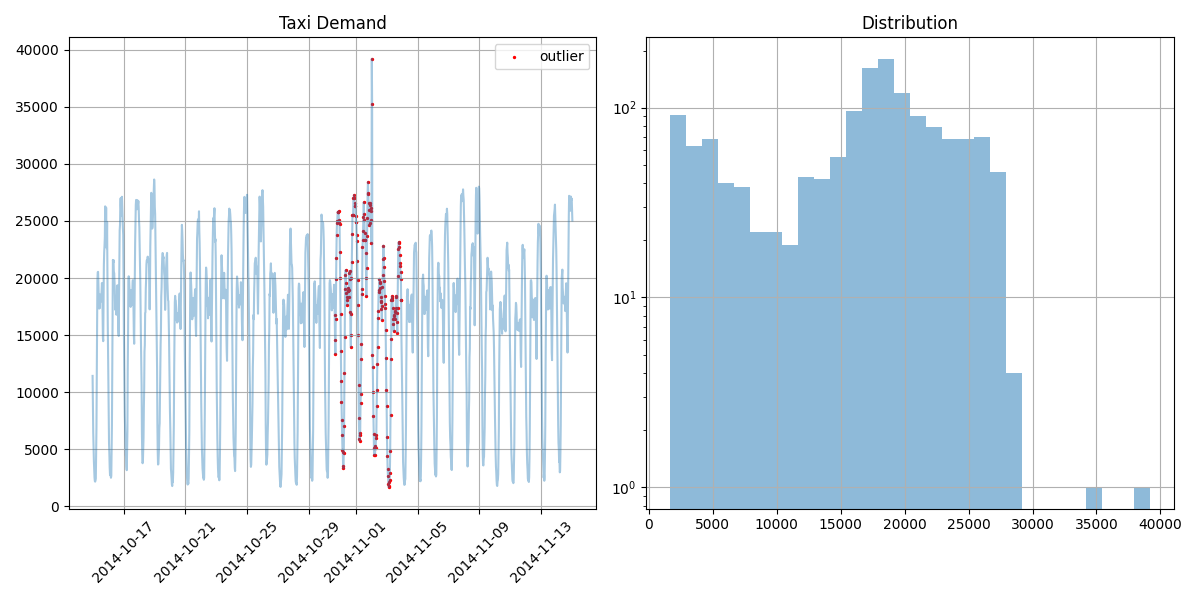
\includegraphics[scale=0.48]{NAB_example_nyc_taxi.png}
    \caption{NYC Taxi demand - anomalies highlighted in red}
    \label{fig:NAB_example_nyc_taxi}
\end{figure}

\subsection{KPI Anomaly Detection Dataset}

The other labeled dataset that we use is the KPI Anomaly Detection Dataset (KPI AIOps) \cite{2208.03938}.
This dataset alongside the NAB dataset will be used to evaluate the predictive performance of the anomaly detection models.

The dataset consists of KPI (key performace index) time series data from many
real scenarios of Internet companies with ground truth label. KPIs fall into two
broad categories: service KPIs and machine KPIs. Service KPIs are performance metrics
that reflect the size and quality of a Web service, such as page response time, page views,
and number of connection errors. Machine KPIs are performance indicators that reflect
the health of the machine (server, router, switch), such as CPU utilization, memory utilization,
disk IO and network card throughput.

A sample time series of a sensor readings is presented in Figure \ref{fig:NAB_example_nyc_taxi}.
We can clearly see the outliers for some of the observations (colored in red).
\begin{figure}[h!]
    \centering
    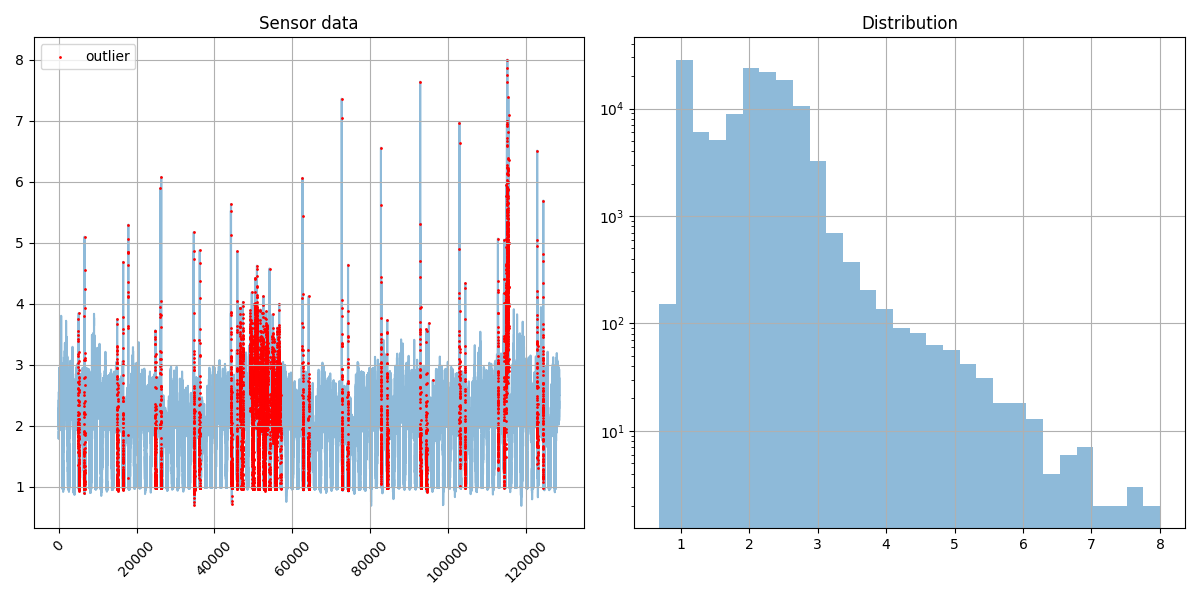
\includegraphics[scale=0.48]{KPIAIOps_example.png}
    \caption{Sensor data from a machine in a data center. The red dots indicate the anomalies.}
    \label{fig:KPIAIOps_example}
\end{figure}

\subsection{FI2010}

In \cite{1705.03233}, authors described the first publicly available benchmark dataset of high-frequency limit order markets for mid-price prediction.
The dataset contains 10-day limit order book data from June 2010 for five stocks that are listed on the Helsinki exchange.
Each entry in the time series provides price details and aggregate order sizes for the top ten levels on both the bid and offer sides of the market,
totaling forty data points. The time series consists of approximately four million messages, representing incoming buy/sell orders or cancellations.
The dataset features order book snapshots taken after every 10 messages, resulting in approximately 400,000 records for the five stocks.

A number of versions of the dataset are available using different normalization schemes. We used the not normalized version of the dataset.

For the purpose of this work, we only extract only the mid price from the dataset which will be used for anomaly detection task.


\subsubsection{Synthetic outliers}

Since the dataset is not labeled, we have to inject synthetic anomalies into the dataset.
We employ the approach similar to \cite{Crepey2022Anomaly} with a slight modification.
The algorithm can be summarized as follows:
\begin{enumerate}
    \item Select $n$ samples from the time series which will be contaminated (i.e., anomalous)
    \item Replace the sample $S_i$ with $\hat{S}_i=S_i(1+\delta)$ where $\delta$ is the injected outlier in the return space.
\end{enumerate}

Authors model $\delta$ as a uniformly distributed random variable $\mathcal{U}[0, \rho]$.
We instead use the normal distribution with matching mean and standard deviation of the returns time series.

An example of the injected outliers is presented in Figure \ref{fig:FI2010_example_outliers_injected}
\begin{figure}[h!]
    \centering
    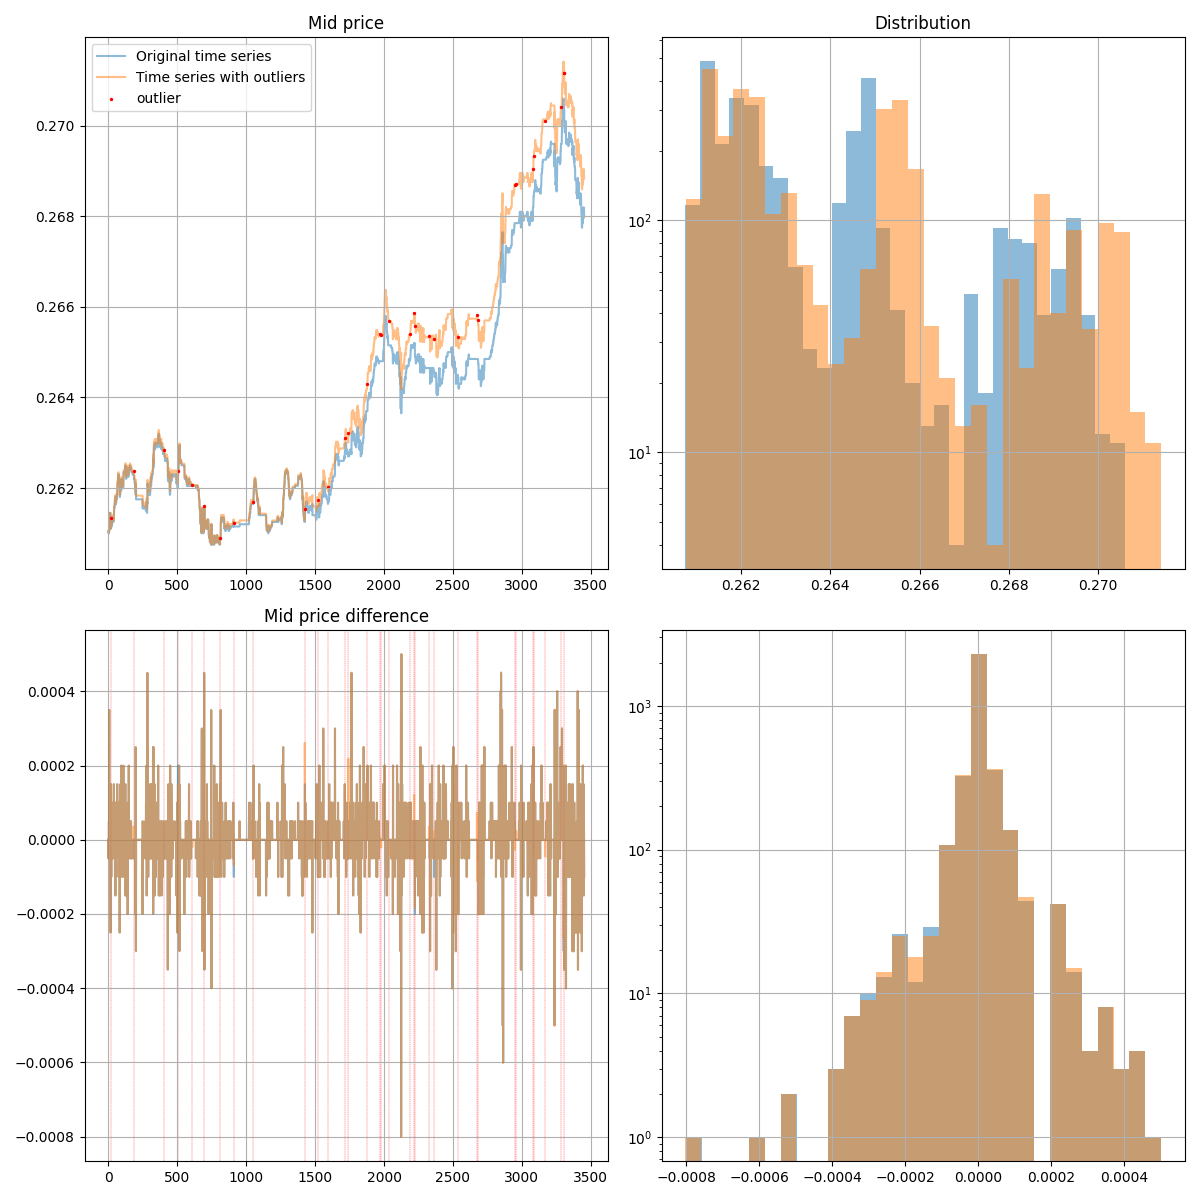
\includegraphics[scale=0.48]{FI2010_example_outliers_injected.png}
    \caption{Example of the injected outliers in the FI2010 dataset.}
    \label{fig:FI2010_example_outliers_injected}
\end{figure}

\section{Accuracy}

TODO: describe the main metrics (accuracy, balanced accuracy, F1, Cohen's Kappa, Confusion matrix)

% for metrics example: https://www.mdpi.com/1999-4893/15/10/385`'

\section{Performance/Speed}

% https://xilinx.github.io/Vitis-Tutorials/2021-2/build/html/docs/Getting_Started/Vitis_HLS/dataflow_design.html

% why pynq has additional latency
% https://discuss.pynq.io/t/execution-time-in-pynq-z2/2833
% https://discuss.pynq.io/t/execution-time-calculation/1959
% In pipeline designs there are two key concepts
% Initiation Interval (II), the number of clock cycles between the start times of consecutive loop iterations, ideally this should be 1
% Latency, the time it takes to get an output since the input was fed



\section{Resource utilization on FPGA}



%%%%%%%%%%%%%%%%%%%%%%%%%%%%%%%%%%%%%%%%%%
\newpage
\chapter*{Conclusion}

\section{Future work}
Bigger FPGA boards.

Evaluation of performance on more recent financial market data.


%%%%%%%%%%%%%%%%%%%%%%%%%%%%%%%%%%%%%%%%%%%%%%%
%%%%%%%%%%%%%%%%%%%%%%%%%%%%%%%%%%%%%%%%%%%%%%%
\newpage
\appendix
\chapter{Code}
\section{Efficient matrix multiplication}\label{app:Appendix}
This is Appendix~\ref{app:Appendix}, which usually contained supporting material,
or complicated proofs that might make the main text above less readable / fluid.

%%%%%%%%%%%%%%%%%%%%%%%%%%%%%%%%%%%%%%%%%%%%%%%
%%%%%%%%%%%%%%%%%%%%%%%%%%%%%%%%%%%%%%%%%%%%%%%
\bibliographystyle{unsrt}
\bibliography{biblio}
\addcontentsline{toc}{chapter}{Bibliography}

\end{document}